\documentclass[Lecture.tex]{subfiles}
\begin{document}
\section{2.7: Bell-Shaped Distributions and Standard Deviations}

\begin{frame}{Standard Deviation}
You can think of the {\it standard deviation} as roughly the average distance that values fall from the mean.
\begin{defn}
The formula for the {\it sample standard deviation} is $$s=\sqrt{\frac{\sum(x-\bar x)^2}{n-1}}$$\pause
The value of $s^2$ is called the {\it sample variance}.
\end{defn}
\end{frame}

\begin{frame}{Example}
Consider the standard deviations for the following sets of data, both with mean 100:\pause
\begin{center}
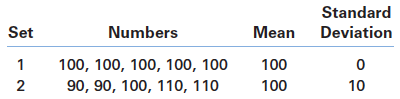
\includegraphics[scale=.5]{standarddev}
\end{center}
\end{frame}

\begin{frame}{The Empirical Rule}
\begin{defn}
The {\it Empirical Rule} states that for any bell-shaped curve, approximately\pause
\begin{itemize}
\item<1->
68\% of the values fall within 1 standard deviation of the mean in either direction,
\item<2->
95\% of the values fall within 2 standard deviations of the mean in either direction,
\item<3->
99.7\% of the values fall within 3 standard deviations of the mean in either direction.
\item<4->
{\bf Note:} A small percentage, about 0.3\%, falls further than 3 standard deviations from the mean.
\end{itemize}
\end{defn}
\end{frame}

\begin{frame}{Standardized z-scores}
\begin{defn}
The {\it standardized score} or {\it z-score} is a useful measure of the relative value of any observation in a dataset.\pause The formula for this score is: $$z=\frac{{\text{Observed value}}-{\text{Mean}}}{{\text{Standard deviation}}}$$
\end{defn}
\end{frame}

\begin{frame}{The Empirical Rule}
We can state the Empirical Rule for any bell-shaped data in terms of $z$-scores:\pause
\begin{center}
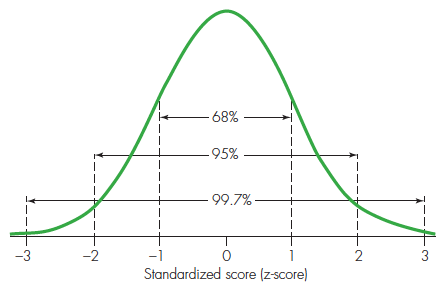
\includegraphics[scale=.5]{empirical}
\end{center}
\end{frame}




\end{document}